% Template for ICASSP-2016 paper; to be used with:
%          spconf.sty  - ICASSP/ICIP LaTeX style file, and
%          IEEEbib.bst - IEEE bibliography style file.
% --------------------------------------------------------------------------
\documentclass[12pt]{article}
\usepackage{spconf,amsmath,graphicx,float}

% Example definitions.
% --------------------
\def\x{{\mathbf x}}
\def\L{{\cal L}}

% Title.
% ------
\title{Predict the Housing Prices in Ames Report}
%
% Single address.
% ---------------
\name{Atom Group: Jifu Zhao (jzhao59), Jinsheng Wang (jwang278)}
\address{Nuclear, Plasma, and Radiological Engineering \\
              University of Illinois at Urbana-Champaign\\
		       Urbana, Illinois 61801, USA}

\begin{document}
%\ninept
%
\maketitle

\section{Introduction}
In this project, our goal is to predict the final price of a home in Ames, Iowa. The data are collected in Ames between 2006 and 2010, which contains 79 explanatory variables about the local homes. The given training dataset has 1460 records in total. And there are 43 categorical variables and 36 numerical variables. 

In this project, we first explore the given training data set. Through some pre-processing methods such as one-hot-encoding and log-transformation, we finally get 287 features. Finally, we applied different models as simple linear regression, Lasso regression and xgboost on the new feature space and predict the house prices. More details are described in the following sections.

\section{Pre-processing}
After exploring the training data set, the first thing we noticed is that, there are some missing values for some features, a summary of missing values is shown in Table \ref{table}.

\begin{table}[htb]
 \caption{Summary of Missing Values} \label{table}
\begin{center}
  \begin{tabular}{  c  c  c }
    \hline
    Feature Name & Data Type & \# of Missing\\ \hline
    LotFrontage    & integer     & 259 \\
    Alley                & factor    & 1369 \\
    MasVnrType    & factor        & 8 \\
    MasVnrArea    & integer        & 8 \\
    BsmtQual        & factor        & 37 \\
    BsmtCond        & factor        & 37 \\
    BsmtExposure    & factor       & 38 \\
    BsmtFinType1    & factor        & 37 \\
    BsmtFinType2    & factor        & 38 \\
    Electrical            & factor        & 1 \\
    FireplaceQu        & factor        & 690 \\
    GarageType        & factor       & 81  \\
    GarageYrBlt        & integer        & 81 \\
    GarageFinish        & factor        & 81 \\
    GarageQual        & factor        & 81 \\
    GarageCond        & factor        & 81 \\
    PoolQC                & factor        & 1453 \\
    Fence                & factor        & 1179 \\
    MiscFeature        & factor        & 1406 \\
    \hline
  \end{tabular}
\end{center}
\end{table}

From Table \ref{table} we can see that, there are 6 features whose missing value is more than $15\%$ of the training set. So, our of first step of pre-processing is to drop those 6 features: LotFrontage, Alley, FireplaceQu, PoolQC, Fence and MiscFeature. 

After dropping those 6 features, for other feature that has missing values, we do the following processing: for numerical value, we replace the missing value with the median of training set, which is the same for the test set. For the categorical data which has missing value, we add a new level of NA for each categorical feature that has missing features. Then, for those categorical feature, it is not a good idea to directly transform them into numerical variables. A  better idea is to transform them into vectors using one-hot-encoding methods. 

After finishing above feature processing, our feature space expands into 287 features in total. With all of these 287 features, we can apply a lot of different models. In this project, we have tried linear regression, Ridge regression, Lasso regression, xgboost model, random forest model and GBM model. After comparing the performance and running time of each model through cross-validation, we finally choose three models: simple linear regression, Lasso regression and xgboost model.

\section{Methods}

\subsection{Linear Regression}
With linear regression, we fit a simple linear model that includes all the variables. During our experiment, we find that, linear regression model is easy and fast to implement. But the result is not as good as other advanced models.

\subsection{Lasso Regression}
In Lasso regression, the best choice of lambda is determined through 10-folder cross-validation and choose the lambda that minimize the cross-validation error. During our experiment, we noticed that, Lasso model perform very good.

\subsection{Random Forest Model}
In random forest model, we use 500 trees and the build model work fun.

%\begin{figure}[htb]
%\centering
%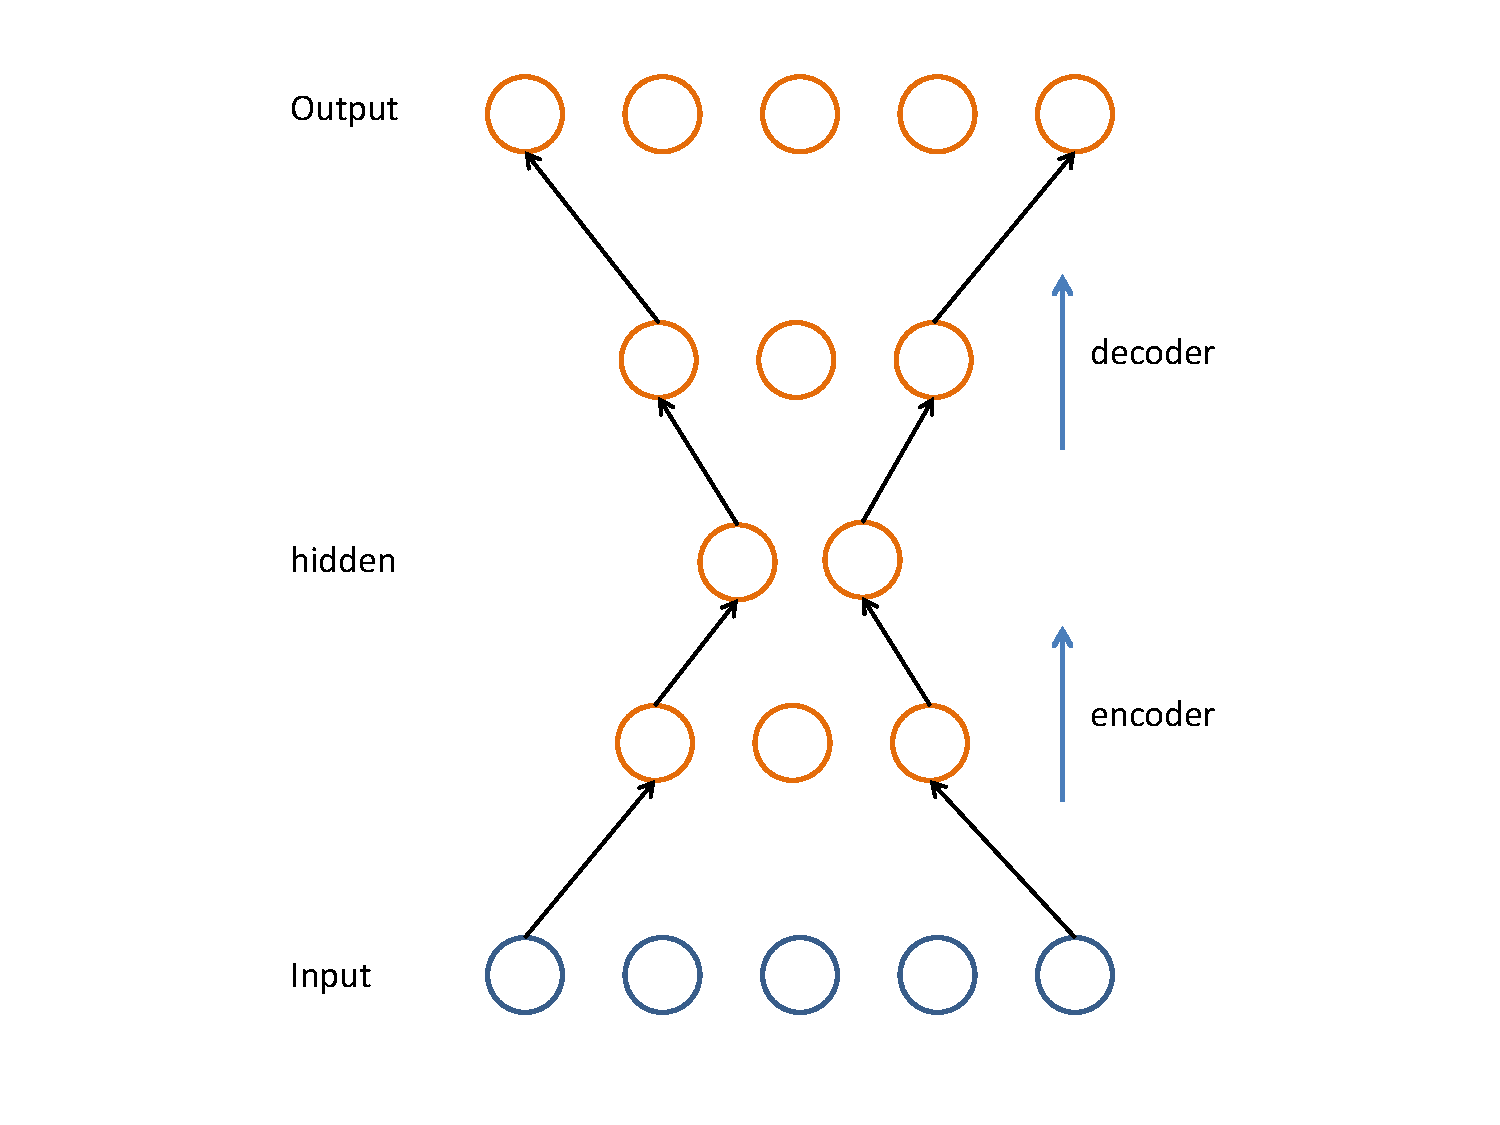
\includegraphics[width=8.5cm]{./figures/autoencoder.pdf}
%\caption{Illustration of auto-encoder system.}
%\label{fig:autoencoder}
%\end{figure}

\section{Code Description}
All of our code is contained in the file named mymain.R. There are basically three parts. On the first part, the code will check whether or not the required packages are already installed. The used package includes dummies, DAAG, randomForest, glmnet, moments. On the second part of the code, we first read the training and test data sets, then drop the useless variables and process the features to form the new feature space. On the third part, we mainly build our three model: linear regression, Lasso regression and random forest model. The built model will make predictions and the results are saved into local file system.

\section{Results}

To test our model, we randomly choose 75\% of data in train.csv as the training set, then use the rest 25\% of data as the test set. This process is repeated 5 times to calculate the average running time, mean-square-error and standard deviation of MSE (MSE is calculated based on log scale). The result of 5 running is shown in Figure \ref{fig:autoencoder}.

\begin{figure}[htb]
\centering
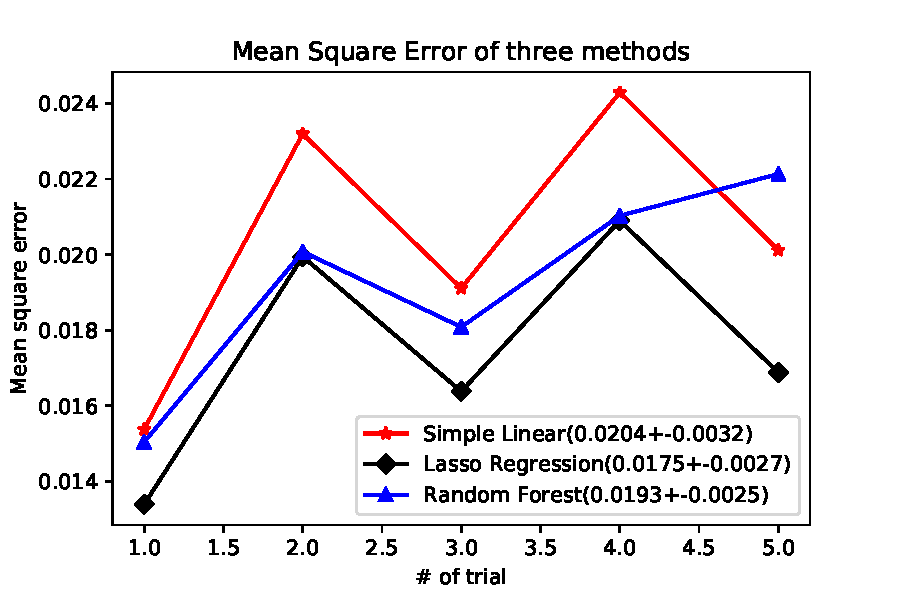
\includegraphics[width=0.45\textwidth]{./figures/MSE_3_methods.pdf}
\caption{Results of different models}
\label{fig:autoencoder}
\end{figure}

The average running time, MSE and standard deviation is shown in Table \ref{result}.

\begin{table}[htb]
 \caption{Summary of Models} \label{result}
\begin{center}
  \begin{tabular}{  c  c c  c }
    \hline
    Model                             & Time(s)              & MSE     & std \\ \hline
    Linear Regression           & 1.3126                               & 0.0204      & 0.0032 \\
    Lasso Regression                & 1.2413                          & 0.0175    & 0.0027 \\
    Random Forest                  & 25.6746                          & 0.0193          & 0.0025 \\
    \hline
  \end{tabular}
\end{center}
\end{table}

From Table \ref{result}, we can find that, Lasso model performs best, and linear regression model performs worst. Lasso and linear model run very fast while random forest runs very slow. 

\subsection*{Acknowledgement}

The authors would like to thank Xichen Huang for his tutorial notebook in Piazza.

\vfill\pagebreak

% References should be produced using the bibtex program from suitable
% BiBTeX files (here: strings, refs, manuals). The IEEEbib.bst bibliography
% style file from IEEE produces unsorted bibliography list.
% -------------------------------------------------------------------------
\bibliographystyle{IEEEbib}
%\bibliography{strings,refs}
\bibliography{strings}

\end{document}
